\documentclass[acmsmall,screen,authorversion]{acmart}

%% \BibTeX command to typeset BibTeX logo in the docs
\AtBeginDocument{
  \providecommand\BibTeX{{
    Bib\TeX}}}

%% Rights management information.  This information is sent to you
%% when you complete the rights form.  These commands have SAMPLE
%% values in them; it is your responsibility as an author to replace
%% the commands and values with those provided to you when you
%% complete the rights form.
\setcopyright{acmcopyright}
\copyrightyear{2023}
\acmYear{2023}
\acmDOI{XXXXXXX.XXXXXXX}

%%
%% These commands are for a JOURNAL article.
%%\acmJournal{JACM}
%%\acmVolume{37}
%%\acmNumber{4}
%%\acmArticle{111}
%%\acmMonth{8}

%%
%% Submission ID.
%% Use this when submitting an article to a sponsored event. You'll
%% receive a unique submission ID from the organizers
%% of the event, and this ID should be used as the parameter to this command.
\acmSubmissionID{XXX-XXX-XXX}

%%
%% For managing citations, it is recommended to use bibliography
%% files in BibTeX format.
%%
%% You can then either use BibTeX with the ACM-Reference-Format style,
%% or BibLaTeX with the acmnumeric or acmauthoryear sytles, that include
%% support for advanced citation of software artefact from the
%% biblatex-software package, also separately available on CTAN.
%%
%% Look at the sample-*-biblatex.tex files for templates showcasing
%% the biblatex styles.
%%

%%
%% The majority of ACM publications use numbered citations and
%% references.  The command \citestyle{authoryear} switches to the
%% "author year" style.
%%
%% If you are preparing content for an event
%% sponsored by ACM SIGGRAPH, you must use the "author year" style of
%% citations and references.
%% Uncommenting the next command will enable that style.
%%\citestyle{acmauthoryear}


\begin{document}

\title[Calysto Scheme]{The Calysto Scheme Project}

\author{James B. Marshall}
\authornote{Both authors contributed equally to this work.}
\affiliation{
  \institution{Sarah Lawrence College}
  \streetaddress{1 Mead Way}
  \city{Bronxville}
  \state{New York}
  \postcode{10708}
  \country{USA}
}
\email{jmarshall@sarahlawrence.edu}

\author{Douglas S. Blank}
\authornotemark[1]
\affiliation{
  \institution{Comet ML, Inc.}
  \city{New York}
  \country{USA}
}
\email{doug.blank@gmail.com}

%% By default, the full list of authors will be used in the page
%% headers. Often, this list is too long, and will overlap other information
%% printed in the page headers. This command allows the author to define a more
%% concise list of authors' names for this purpose.
\renewcommand{\shortauthors}{D. S. Blank and J. B. Marshall}

\begin{abstract}
The abstract goes here. The abstract goes here. The abstract goes here. The
abstract goes here. The abstract goes here. The abstract goes here. The
abstract goes here. The abstract goes here. The abstract goes here. The
abstract goes here. The abstract goes here. The abstract goes here. The
abstract goes here. The abstract goes here. The abstract goes here. The
abstract goes here. The abstract goes here. The abstract goes here. The
abstract goes here. The abstract goes here. The abstract goes here.
\end{abstract}

%% The code below is generated by the tool at http://dl.acm.org/ccs.cfm.
%% Please copy and paste the code instead of the example below.
%%
\begin{CCSXML}
<ccs2012>
<concept>
<concept_id>10011007.10011006.10011008</concept_id>
<concept_desc>Software and its engineering~General programming languages</concept_desc>
<concept_significance>500</concept_significance>
</concept>
<concept>
<concept_id>10011007.10011006.10011008.10011009.10011012</concept_id>
<concept_desc>Software and its engineering~Functional languages</concept_desc>
<concept_significance>500</concept_significance>
</concept>
<concept>
<concept_id>10011007.10011006.10011066.10011069</concept_id>
<concept_desc>Software and its engineering~Integrated and visual development environments</concept_desc>
<concept_significance>500</concept_significance>
</concept>
</ccs2012>
\end{CCSXML}

\ccsdesc[500]{Software and its engineering~General programming languages}
\ccsdesc[500]{Software and its engineering~Functional languages}
\ccsdesc[500]{Software and its engineering~Integrated and visual development environments}

%% Keywords. The author(s) should pick words that accurately describe
%% the work being presented. Separate the keywords with commas.
\keywords{Scheme, Python, Jupyter, whatever}

\received{14 July 2023}
\received[revised]{..........}
\received[accepted]{..........}

%% This command processes the author and affiliation and title
%% information and builds the first part of the formatted document.
\maketitle

\section{Introduction}

This paper describes the development of Calysto Scheme, a fully-featured
implementation of the Scheme programming language written in Scheme, which can
be automatically translated into other languages, such as Python and C\#
\cite{CalystoScheme}.  Although our path through the development of this system
was circuitous, the completed project ended up being far more interesting (and
useful) than we could have imagined.

The initial motivation for Calysto Scheme grew out of an earlier open-source
project called Calico that was designed to be a multi-programming-language
framework and learning environment for computing education \cite{Calico}.  The
basic premise of this earlier project was to create a common architecture, user
interface, and set of libraries for a variety of programming languages (see
Figure~\ref{fig:calico}).

Many engaging ``pedagogical contexts'' for learning about
computer science have been developed, including media computation
\cite{Guzdial03}, gaming, AI and robotics \cite{Myro}, visualization, music,
and art.  However, these contexts often depend on a set of libraries developed
for a specific programming language, which may constrain the choice of language
if an instructor wishes to have students explore a particular learning
context. Having a common framework separates the details of a specific language
from other pedagogical goals.

One of the interesting aspects of Calico was that instead of having
students learn a different IDE for each language under study, such as
IDLE for Python, or DrRacket for Scheme, students could remain in the
same IDE, but simply switch the programming language. This is similar
in spirit to the way that one can switch languages in
DrRacket. However, in Calico, supported languages need not share much
at all with each other.

At the time (2007), Microsoft had embarked on a somewhat-related
goal. They were actively developing what they called the Dynamic
Language Runtime (DLR) as part of the .NET framework [DLR]. The DLR
abstraction layer created a common API and allowed one to create
languages, such as IronPython and IronRuby \cite{IronRuby}, without
having to rewrite the common parts for each language. Our earlier
project adopted the DLR as its foundation, and used these Iron
languages. In addition, the Calico team developed other languages to
augment these, including a visual block-based language.

However, there was a gap in the languages available: there was no
Scheme implementation that could work in this environment. Although
the development of both IronLisp and IronScheme \cite{IronScheme} had
been attempted by other groups, they both ultimately failed for
various reasons, including lack of support for tail-call optimization
(TCO) in the DLR.\footnote[1]{IronScheme eventually did include at
least some support for first-class continuations. However, it was
incrementally added beginning in late 2008
\cite{IronScheme-Continuations} after we had begun building Calysto
Scheme.}

Of course, the Scheme language can be implemented in languages without
TCO. So, we set out to fill this void by developing a Scheme without
using the DLR for internal function calls, but still allowing
integration with the DLR for interoperation with other functionality
(such as calling libraries). Thus, we began the development of what
would become Calysto Scheme.

Once the core Scheme language was written in Scheme (as described below), the
final conversion step to C\# was relatively straightforward. At this point, we
were able to add Scheme to our list of supported languages, including Python,
F\#, and Ruby.  The code snippets in Figure~\ref{fig:scripts} show demo scripts
written in each language, all of which call functions from the same underlying
graphics library. Each script creates a graphics window titled ``Hello'', and
draws a line between (0,0) and (100, 100). Although the calls to library
functions in each language differ merely in their syntax, there are many deeper
differences between the languages in terms of semantics.

Although we initially targeted C\# as the implementation language, we
eventually decided to replace C\# with Python (see below). The core Calysto
Scheme architecture remained the same, only the final transformation step
needed to be changed to target Python rather than C\#. The transformation to
Python also included changing calls to C\#'s DLR to calls to standard Python
functions. The following section outlines the overall Calysto Scheme design
pipeline.

%---------------------------------------------------------------------------------

\begin{figure}
  \centering
  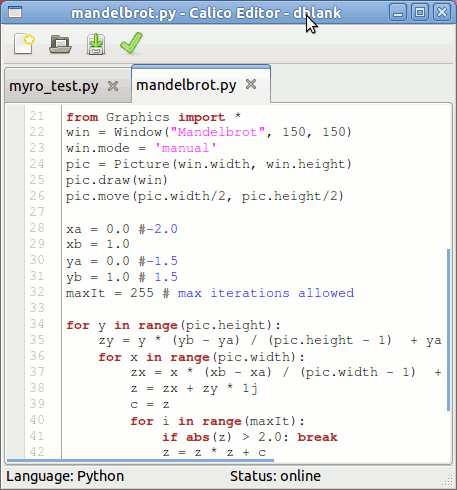
\includegraphics[width=0.40\textwidth]{calico-interface-python.jpg}
  \hspace{0.15in}
  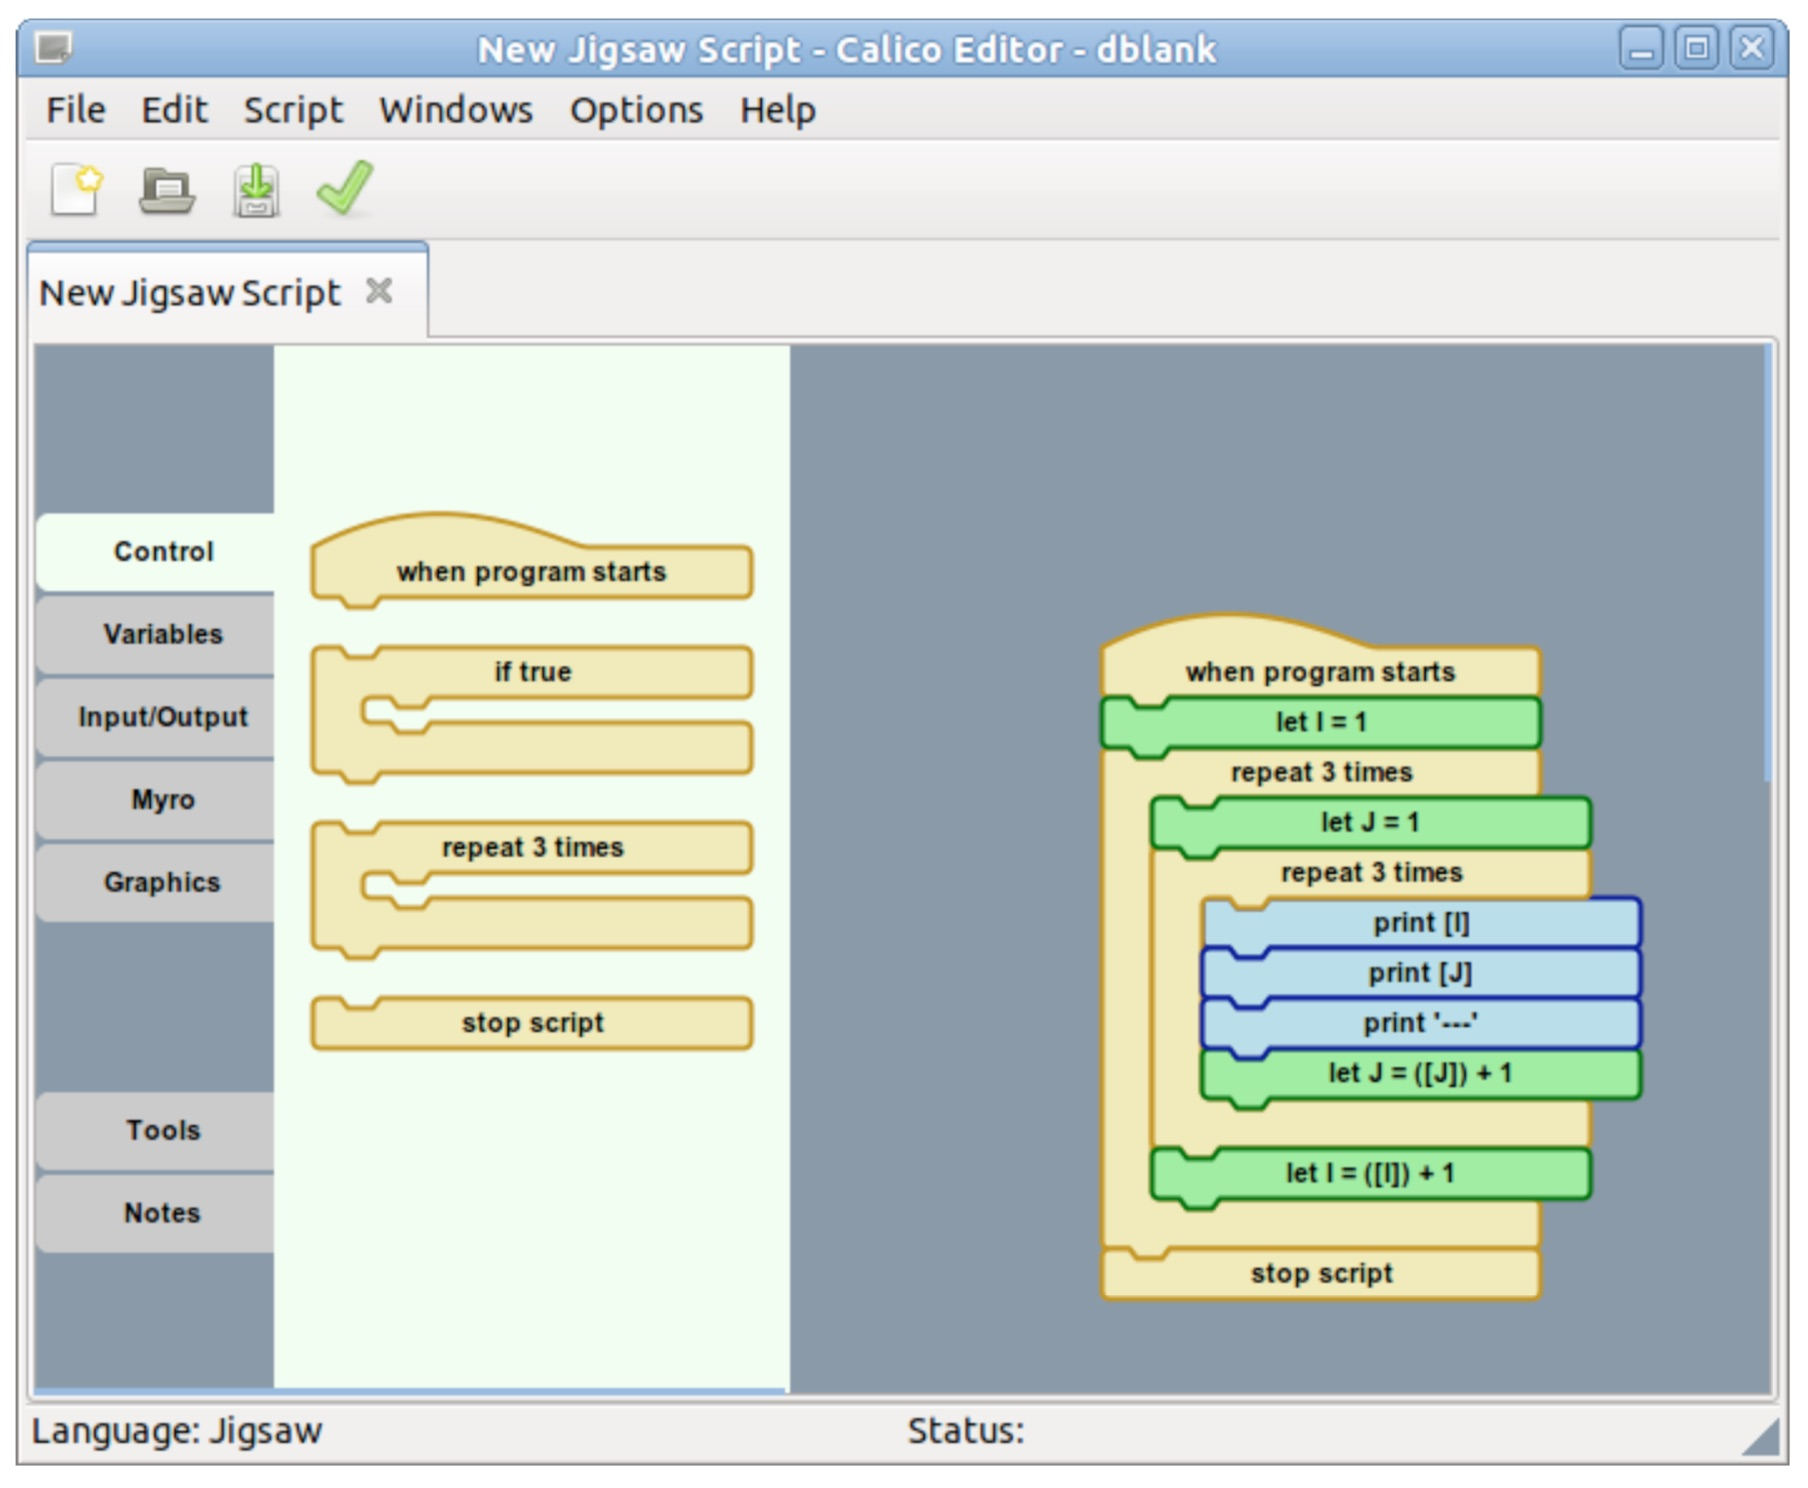
\includegraphics[width=0.523\textwidth]{calico-interface-jigsaw.jpg}
  \caption{The Calico interface, running Python (left),
    and Jigsaw, a visual block-based language (right).}
  \label{fig:calico}
  \Description{User interface windows showing code written in Python and code
    written in a visual block-based language.}
\end{figure}

%---------------------------------------------------------------------------------

\begin{figure}
  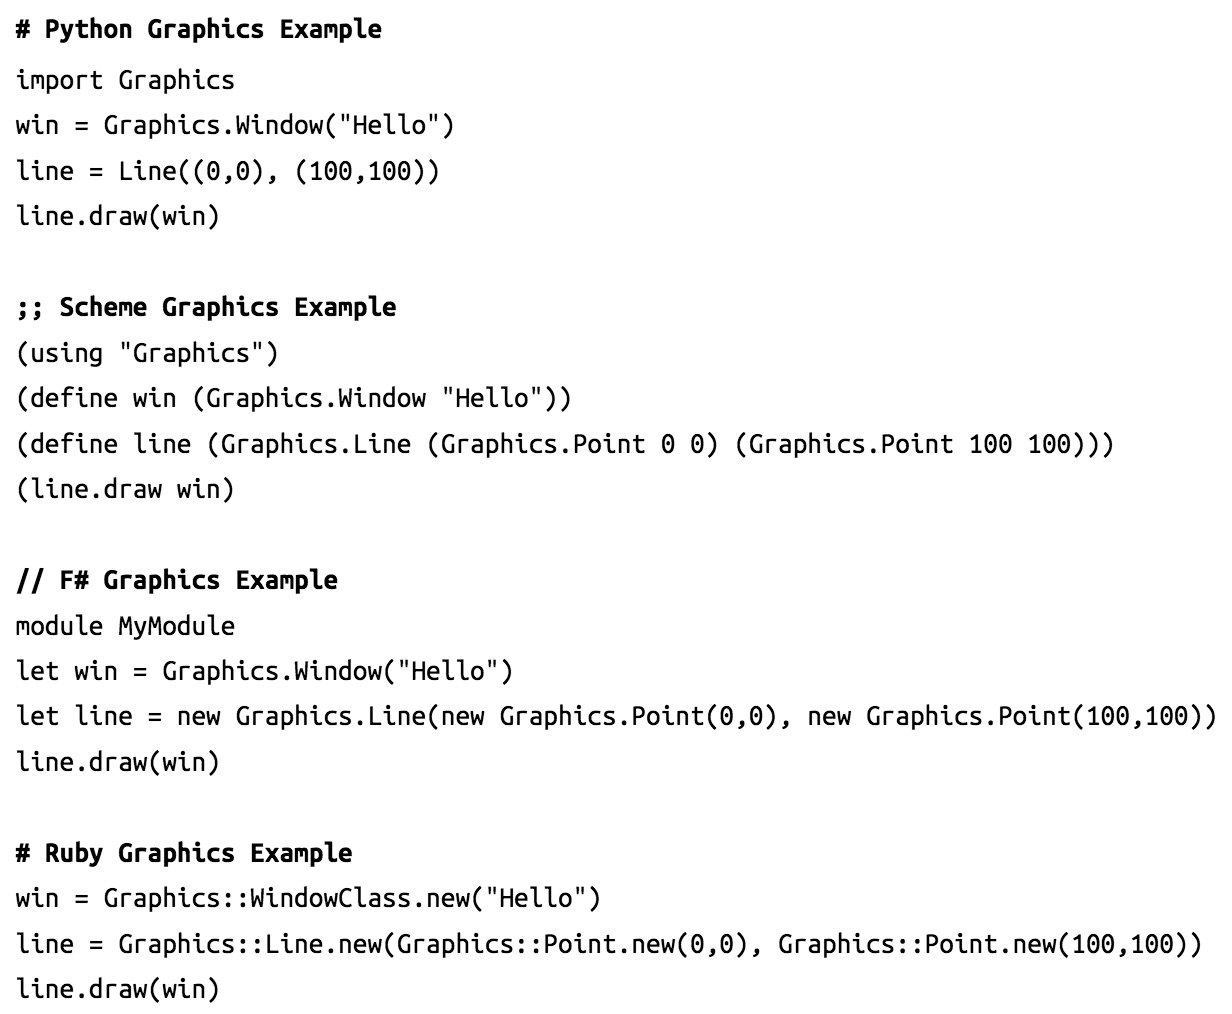
\includegraphics[width=0.7\textwidth]{graphics-scripts.jpg}
  \caption{Calling the same graphics library functions from four different languages in Calico.}
  \label{fig:scripts}
  \Description{}
\end{figure}

%---------------------------------------------------------------------------------

\begin{figure}
\begin{minipage}{0.4\textwidth}
{\scriptsize
\begin{verbatim}
;; global registers
(define n_reg 'undefined)
(define k_reg 'undefined)
(define value_reg 'undefined)
(define fields_reg 'undefined)
(define pc 'undefined)
(define final_reg 'undefined)

(define trampoline
  (lambda ()
    (if pc
        (begin
          (pc)
          (trampoline))
        final_reg)))

(define make-cont
  (lambda args
    (cons 'continuation args)))

(define apply-cont
  (lambda ()
    (let ((label (cadr k_reg))
          (fields (cddr k_reg)))
      (set! fields_reg fields)
      (set! pc label))))

(define <cont-1>
  (lambda ()
    (set! final_reg value_reg)
    (set! pc #f)))

(define <cont-2>
  (lambda ()
    (let ((n (car fields_reg))
          (k (cadr fields_reg)))
      (set! k_reg k)
      (set! value_reg (+ n value_reg))
      (set! pc apply-cont))))

(define sum-cps
  (lambda ()
    (if (= n_reg 0)
      (begin
        (set! value_reg 0)
        (set! pc apply-cont))
      (begin
          (set! k_reg (make-cont <cont-2> n_reg k_reg))
        (set! n_reg (- n_reg 1))
        (set! pc sum-cps)))))

;; top-level function
(define sum
  (lambda (n)
    (set! k_reg (make-cont <cont-1>))
    (set! n_reg n)
    (set! pc sum-cps)
    (trampoline)))







\end{verbatim}
}
\caption{Scheme register machine code}
\label{fig:schemeRM}
\end{minipage}
\hspace{0.75in}
\begin{minipage}{0.4\textwidth}
{\scriptsize
\begin{verbatim}
# global registers
n_reg = None
k_reg = None
value_reg = None
fields_reg = None
pc = None
final_reg = None

def trampoline():
    while pc:
        pc()
    return final_reg

def car(lst):
    return lst[0]

def cdr(lst):
    return lst[1:]

def cadr(lst):
    return car(cdr(lst))

def cddr(lst):
    return cdr(cdr(lst))

def make_cont(*args):
    return ("continuation",) + args

def apply_cont():
    global fields_reg, pc
    label = cadr(k_reg)
    fields = cddr(k_reg)
    fields_reg = fields
    pc = label

def cont_1():
    global final_reg, pc
    final_reg = value_reg
    pc = False

def cont_2():
    global k_reg, value_reg, pc
    n = car(fields_reg)
    k = cadr(fields_reg)
    k_reg = k
    value_reg = n + value_reg
    pc = apply_cont

def sum_cps():
    global value_reg, pc, k_reg, n_reg
    if n_reg == 0:
        value_reg = 0
        pc = apply_cont
    else:
          k_reg = make_cont(cont_2, n_reg, k_reg)
        n_reg = n_reg - 1
        pc = sum_cps

# top-level function
def sum(n):
    global k_reg, n_reg, pc
    k_reg = make_cont(cont_1)
    n_reg = n
    pc = sum_cps
    return trampoline()
\end{verbatim}
}
\caption{Python register machine code}
\label{fig:pythonRM}
\end{minipage}
\end{figure}

%---------------------------------------------------------------------------------

\section{Calysto Scheme Design}

Calysto Scheme ensures full support for tail-call optimization, with no limit
placed on the depth of the call stack.  Unfortunately, languages such as C\#
and Python impose a maximum depth on their recursion stack and do not support
tail-call optimization.  Therefore, our approach was to implement the Calysto
Scheme interpreter in Scheme, and then automatically convert it, via a series
of correctness-preserving program transformations, into low-level register
machine code that does not rely on the recursion stack, which can then be
directly transformed into Python (or C\#) as the final step.  The high-level
Scheme version of the interpreter is written in continuation-passing style
(CPS), with continuations initially represented as anonymous lambda functions.
The continuations are then converted to a data structure representation (as
lists), and from there passing information to functions via arguments is
replaced by passing information via a set of global registers, which removes
the reliance on the call stack.  At this stage, the computation is driven by a
single ``trampoline'' loop, essentially equivalent to a while loop
\cite{Ganz99, EOPL3}.

As an example of the transformation process, consider a simple recursive
function that adds up the first $n$ positive integers.  We start with a version
of this function written in CPS, using functional continuations, as shown
below.  For example, calling the top-level function \texttt{(sum 100)} returns
5050.

{\small
\begin{verbatim}
(define sum-cps
  (lambda (n k)
    (if (= n 0)
        (k 0)
        (sum-cps (- n 1)
          (lambda (value)
            (k (+ n value)))))))

;; top-level function
(define sum
  (lambda (n)
    (sum-cps n (lambda (value) value))))

\end{verbatim}
}

\noindent
We wrote a program that takes any Scheme program written in CPS, such as the
above, and transforms the code into an equivalent register machine, with
continuations represented as lists.  The resulting register machine for
\texttt{sum} is shown in Figure~\ref{fig:schemeRM}.  Calling \texttt{(sum 100)}
still returns 5050, as before.

At this stage, all functions other than the trampoline simply execute
if-statements or update registers via assignment statements, without ever
calling another function directly (except for low-level built-in primitives
like \texttt{car} or \texttt{+}).  This avoids building up chains of function
calls.  This code can then be directly converted into Python (see
Figure~\ref{fig:pythonRM}).  Since the Python version of \texttt{sum} is no
longer constrained by the depth of the recursion stack, it can be called with
arbitrarily large values of $n$.

In a similar fashion, we transform our Calysto Scheme interpreter from a
high-level recursive CPS program written in Scheme into an equivalent low-level
register machine written in Python, which does not grow Python's call stack.

There is an interesting aspect to creating a language in this manner: the
implementation can be tested at each stage of the transformation process to
ensure correctness. That is, the same suite of Scheme test programs can be run
independently with the CPS, Data Structure, Register Machine, and Python
implementations. In essence, the initial CPS definition serves as both a
high-level language specification and an executable implementation of the
language, from which the other three implementations are subsequently
derived. This allows us to test each stage separately to catch bugs in the CPS
specification and the transformation process itself.

The current version of Calysto Scheme requires an existing Scheme
implementation to carry out the transformations from CPS to Data Structures,
and from Data Structures to Register Machine.  The final conversion from Scheme
to Python is written in Python.  We used Petite Chez Scheme in early
development, and switched to Chez Scheme when it was made open source. In
principle, it would be possible to make Calysto Scheme self-hosting
(\emph{i.e.}, Calysto Scheme could carry out the transformations
itself). However, our transformation program currently relies on Chez Scheme's
\texttt{syntax-rules} macro definition facility, which differs somewhat from
the version of \texttt{define-syntax} implemented in Calysto Scheme.

%%However, our transformation program takes advantage of Chez Scheme's
%%version of \texttt{define-syntax}, which is more advanced than the version
%%currently implemented in Calysto Scheme.

\section{Syntactic Extension}

\noindent
Calysto Scheme supports syntactic extension through its own version of
\texttt{define-syntax}, which can define simple macros using standard list
notation in conjunction with unification pattern matching variables that
begin with the \texttt{?} character.  For example, consider the following
macro expansion rules for \texttt{and} and \texttt{or} expressions:\\

\begin{minipage}{\textwidth}
\texttt{(and $\mathit{exp}$)} $~\rightarrow~$ $\mathit{exp}$\\
\texttt{(and $\mathit{exp}_1~\mathit{exp}_2~\mathit{exp}_3~\ldots$)} $~\rightarrow~$
\texttt{(if $\mathit{exp}_1$ (and $\mathit{exp}_2~\mathit{exp}_3~\ldots$) \#f)}\\

\texttt{(or $\mathit{exp}$)} $~\rightarrow~$ $\mathit{exp}$\\
\texttt{(or $\mathit{exp}_1~\mathit{exp}_2~\mathit{exp}_3~\ldots$)} $~\rightarrow~$
\texttt{(if $\mathit{exp}_1$ \#t (or $\mathit{exp}_2~\mathit{exp}_3~\ldots$))}\\
\end{minipage}

\noindent
Although \texttt{and} and \texttt{or} are already available in Calysto Scheme,
in principle they could be implemented with the following recursive macro
definitions:

\begin{verbatim}
(define-syntax and
  [(and ?exp) ?exp]
  [(and ?first-exp . ?other-exps) (if ?first-exp (and . ?other-exps) #f)])


(define-syntax or
  [(or ?exp) ?exp]
  [(or ?first-exp . ?other-exps) (if ?first-exp #t (or . ?other-exps))])
\end{verbatim}

\section{Nondeterministic Backtracking}

\noindent
In their classic text \emph{Structure and Interpretation of Computer Programs}
(SICP) \cite{SICP}, Abelson and Sussman introduce the nondeterministic ``amb''
operator for automatic backtracking.  We have incorporated this operator into
Calysto Scheme as the special form
\texttt{(choose~$\mathit{arg}_1~\mathit{arg}_2~\ldots~\mathit{arg}_n$)}, which
nondeterministically chooses one of its arguments to evaluate and returns the
resulting value.  From there, the computation proceeds normally, unless
\texttt{(choose)} is subsequently invoked with no arguments, at which point the
computation ``fails'' and immediately jumps back to the previous
\texttt{choose} expression, whereby a different argument is chosen to evaluate
next, and the computation restarts from that point with the new value.  Many
constraint-satisfaction problems can be elegantly solved using \texttt{choose}.

As an example illustrating both \texttt{choose} and
\texttt{define-syntax}, suppose we wish to write a program to determine how to
color a map of (a portion of) Western Europe using four distinct colors.  We
first define a function to nondeterministically return one of four possible
colors:

{\small
\begin{verbatim}
(define choose-color
  (lambda ()
    (choose 'red 'yellow 'blue 'white)))
\end{verbatim}
}

\noindent
The \texttt{color-europe} program begins by nondeterministically assigning a
color to each country on the map:

{\small
\begin{verbatim}
(define color-europe
  (lambda ()
    (let ([portugal (choose-color)]
          [spain (choose-color)]
          [france (choose-color)]
          [belgium (choose-color)]
          [germany (choose-color)]
          [luxembourg (choose-color)]
          [italy (choose-color)]
          [switzerland (choose-color)])
        ...)))
\end{verbatim}
}

\noindent
Next, we must apply the following constraint to each country: its chosen color
must be different from that of all of its adjacent neighbors.  For example,
since Luxembourg is bordered by France, Belgium, and Germany, we could express
its color constraint as follows:

{\small
\begin{verbatim}
(require (not (member luxembourg (list france belgium germany))))
\end{verbatim}
}

\noindent
The \texttt{require} function is a Calysto Scheme primitive similar to an
assertion statement, which takes a boolean value as input and invokes
\texttt{(choose)} if the input is false in order to force the program to
backtrack to the most recent choice point, instead of raising an exception.
However, a more elegant approach might be to define a new syntactic form called
\texttt{color} that expresses this constraint in a very readable way:

{\small
\begin{verbatim}
(color luxembourg different from france belgium germany)
\end{verbatim}
}

\noindent
The Calysto Scheme macro definition for \texttt{color}, along with the complete
program to determine a consistent map-coloring, is given below:

%\noindent
%\begin{minipage}{\textwidth}
{\small
\begin{verbatim}
(define-syntax color
  [(color ?country different from . ?neighbors)
   (require (not (member ?country (list . ?neighbors))))])
\end{verbatim}
}
%\end{minipage}

\noindent
\begin{minipage}{\textwidth}
{\small
\begin{verbatim}
(define color-europe
  (lambda ()
    (let ([portugal (choose-color)]
          [spain (choose-color)]
          [france (choose-color)]
          [belgium (choose-color)]
          [germany (choose-color)]
          [luxembourg (choose-color)]
          [italy (choose-color)]
          [switzerland (choose-color)])
      ;; apply the constraints
      (color portugal different from spain)
      (color spain different from france portugal)
      (color france different from spain italy switzerland belgium germany luxembourg)
      (color belgium different from france luxembourg germany)
      (color germany different from france switzerland belgium luxembourg)
      (color luxembourg different from france belgium germany)
      (color italy different from france switzerland)
      (color switzerland different from france italy germany)
      ;; return a coloring that satisfies the constraints
      (list (list 'portugal portugal)
            (list 'spain spain)
            (list 'france france)
            (list 'belgium belgium)
            (list 'germany germany)
            (list 'luxembourg luxembourg)
            (list 'italy italy)
            (list 'switzerland switzerland)))))

\end{verbatim}
}
\end{minipage}

\noindent
Calling \texttt{(color-europe)} returns the solution \texttt{((portugal red)
  (spain yellow) (france red) (belgium yellow) (germany blue) (luxembourg
  white) (italy yellow) (switzerland white))}. However, this is not the only
valid solution; many other color combinations will work.  We can force the
program to backtrack to find another combination that satisfies the
constraints, simply by calling \texttt{(choose)} as many times as we like,
until all valid choices have been returned:

{\small
\begin{verbatim}
==> (choose)
((portugal red) (spain yellow) (france red) (belgium yellow) (germany blue)
 (luxembourg white) (italy blue) (switzerland yellow))
==> (choose)
((portugal red) (spain yellow) (france red) (belgium yellow) (germany blue)
 (luxembourg white) (italy blue) (switzerland white))
\end{verbatim}
}

\noindent
and so on.  Eventually, after all possible combinations of choices that satisfy
the constraints have been returned, any subsequent calls to \texttt{(choose)}
will return the string ``no more choices'', until a new \texttt{choose}
expression is executed.

\section{Python / Scheme Interoperation}

There are a number of ways that Calysto Scheme and Python can interoperate. For
example, Python code can be directly evaluated from within Scheme. Scheme
functions can be defined in an environment shared with Python, and then called
by Python programs. And Python functions and libraries can be imported directly
into Scheme and called from within Scheme programs.

Whereas in Scheme everything is an expression, Python makes a distinction
between evaluation and execution. In Calysto Scheme, the function
\texttt{python-eval} can be used to evaluate strings representing Python
expressions, and \texttt{python-exec} can be used to execute Python
statements.\\

{\small
\noindent
\texttt{(python-eval "1 + 2")}\\
$\rightarrow$ 3

\noindent
\begin{verbatim}
(python-exec
"
def mypyfunc(a, b):
    return a * b
")
\end{verbatim}
\noindent\texttt{(python-eval "mypyfunc(2, 3)")}\\
$\rightarrow$ 6\\
}

\noindent
The special form \texttt{func} turns a Scheme procedure into a Python function,
and \texttt{define!} puts it into the shared environment with Python:\\

{\small
\noindent
\texttt{(define! mypyfunc2 (func (lambda (n) (* n n))))}\\
\texttt{(python-eval "mypyfunc2(3)")}\\
$\rightarrow$ 9\\
}

\noindent
As a simple illustration of Calysto Scheme's ability to import and use
functions from Python and its libraries, consider the following example, in
which the elements of a nested Scheme list are summed by converting it into a
Numpy array and then applying the Numpy \texttt{sum} function:\\

\begin{minipage}{\textwidth}
{\small
\begin{verbatim}
(import "numpy")

(let ([matrix3d '(((10 20 30) (40 50 60))
                  ((70 80 90) (100 110 120))
                  ((130 140 150) (160 170 180))
                  ((190 200 210) (220 230 240)))])
  (numpy.sum (numpy.array matrix3d)))
\end{verbatim}
$\rightarrow$ 3000\\
}
\end{minipage}

\noindent
Python dictionaries can also be created and manipulated from within Calysto
Scheme using a special syntax, as shown in the example interaction below:\\

\begin{minipage}{\textwidth}
{\small
\begin{verbatim}
==> (define d (dict '((apple : red) (banana : yellow) (lime : green))))
==> d
{'apple': red, 'banana': yellow, 'lime': green}
==> (get-item d 'apple)
red
==> (set-item! d 'apple 77)
==> d
{'apple': 77, 'banana': yellow, 'lime': green}
\end{verbatim}
}
\end{minipage}

%\section{A Modern Example}

\noindent
\\\\A more complex example that shows the power of combining these features is
shown in Figure~\ref{fig:tensorflow}. This Scheme code sets up a series of
machine learning experiments using the Numpy and Tensorflow libraries imported
from Python, along with a third-party library called \texttt{comet\_ml} that
provides tools for managing experiments.  The \texttt{choose} operator is used
to select a particular combination of ``hyperparameters'' for an experiment,
and a neural network is then defined using Tensorflow functions.  Many
Tensorflow functions are configured via keyword parameters in Python, which
here we provide as Calysto Scheme dictionaries.  After an experiment using a
particular set of hyperparameters has run to completion, we can simply invoke
\texttt{(choose)} to pick a new combination of hyperparameters and rerun the
experiment.

%---------------------------------------------------------------------------------

\begin{figure}
\begin{minipage}{0.8\textwidth}
{\scriptsize
\begin{verbatim}
(import-as "tensorflow" "tf")
(import-as "numpy" "np")
(import "comet_ml")

;; load the MNIST dataset using the Keras load_data function
(define dataset (tf.keras.datasets.mnist.load_data))

;; prepare the dataset
(define x_train (/ (get-item (get-item dataset 0) 0) 255.0))
(define y_train (get-item (get-item dataset 0) 1))
(define x_test (/ (get-item (get-item dataset 1) 0) 255.0))
(define y_test (get-item (get-item dataset 1) 1))

(define loss_fn (tf.keras.losses.SparseCategoricalCrossentropy (dict '((from_logits : #t)))))

(let* ([optimizer (choose "adam" "rmsprop" "sgd")]
       [dropout_rate (choose 0.0 0.1 0.2 0.4)]
       [activation (choose "relu" "sigmoid")]
       [hidden_layer_size (choose 10 20 30)]
       [options (dict `((optimizer : ,optimizer)
                        (loss : ,loss_fn)
                        (metrics : ,(vector "accuracy"))))]
       [epochs 5]
       [experiment (comet_ml.Experiment (dict '((project_name : "calysto-scheme"))))]
       [model (tf.keras.models.Sequential 
                (vector
                 (tf.keras.layers.Flatten (dict '((input_shape : (28 28)))))
                     (tf.keras.layers.Dense hidden_layer_size (dict `((activation : ,activation))))
                 (tf.keras.layers.Dropout dropout_rate)
                 (tf.keras.layers.Dense 10)))])
  (print experiment.url)
  (model.compile options)
  (model.summary)
  (experiment.log_parameters (dict `((optimizer : ,optimizer)
                                     (dropout_rate : ,dropout_rate)
                                     (activation : ,activation)
                                     (hidden_layer_size : ,hidden_layer_size)
                                     (epochs : ,epochs)))
                             (dict))
  (experiment.set_model_graph model)
  (let ([history (model.fit x_train y_train (dict `((epochs : ,epochs))))]
        [step 0])
    (map (lambda (key)
           (set! step 0)
           (map (lambda (v)
                  (experiment.log_metric key v step)
                  (set! step (+ step 1)))
                (get-item history.history key)))
         history.history))
  (experiment.end))
\end{verbatim}
}
\end{minipage}
\caption{Calysto Scheme code for running Tensorflow experiments.}
\label{fig:tensorflow}
\end{figure}

%---------------------------------------------------------------------------------

\section{Calysto Scheme in Jupyter}

The Jupyter Project is a language-independent client-server system for
running code using a web browser as the IDE
\cite{Kluyver2016jupyter}. Initially, Jupyter was limited to Python
(and was originally called IPython \cite{PER-GRA:2007}). However, the
developers realized that their system could be used for any language,
and the Jupyter Project was born. Today, Jupyter is one of the
most-used tools in data science. Jupyter Notebooks allow the mixing of
code, text, mathematics, and visualizations within a single executable
document.

In many ways, the goals of Jupyter were similar to the original goals of
Calysto Scheme: language independence with a common UI. In fact, when Jupyter
was announced, we realized that this made more sense than our C\#-based system,
and we began migration of our project to the Jupyter framework. Calysto Scheme,
in fact, gets its name from Callisto, the second largest moon of the planet
Jupiter.

Running Calysto Scheme in a Jupyter environment (such as notebook, jupyterlab,
console, or qtconsole) provides the following additional features:

\begin{itemize}
\item TAB completions of Scheme functions and variable names
\item Ability to directly display rich media such as images
\item Access to so-called magics (\texttt{\%} meta commands)
\item Ability to easily run shell commands (using the ``\texttt{!} command'' format)
\item \LaTeX-style equations and variables
\item Additional Python integration
\end{itemize}

For example, in Calysto Scheme running in Jupyter, one can create a lambda
function with the Greek symbol $\lambda$ in place of the \texttt{lambda}
keyword by typing \textbf{\textbackslash lambda} and pressing [TAB] (see
Figure~\ref{fig:fact1}). Building on top of the Jupyter system makes Calysto
Scheme easy to use, and brings it into a modern language environment.

It should be noted that many computer science educators find the use
of Jupyter Notebooks problematic. The main objection is that it is
easy for a student to create hidden state that creates a non-intuitive
experience. For example, one can edit cells that have already been
executed, creating dependencies that are no longer valid. In spite of
this limitation, Jupyter Notebooks are popular with data scientists
and others who tell stories with code, visualizations, and text. For
more on this topic, see \cite{Calico2}.

Judging from the Calysto Scheme github reported issues, most people discover
Calysto Scheme through the Jupyter Project's ``Try Jupyter'' page where Calysto
Scheme is featured along with kernels in C++, Julia, GNU Octave, R, and Ruby
\cite{TryJupyter}. Many people apparently use Calysto Scheme for working
through SICP exercises. See Figure~\ref{fig:try-jupyter}.

\begin{figure}[h]
  \centering
  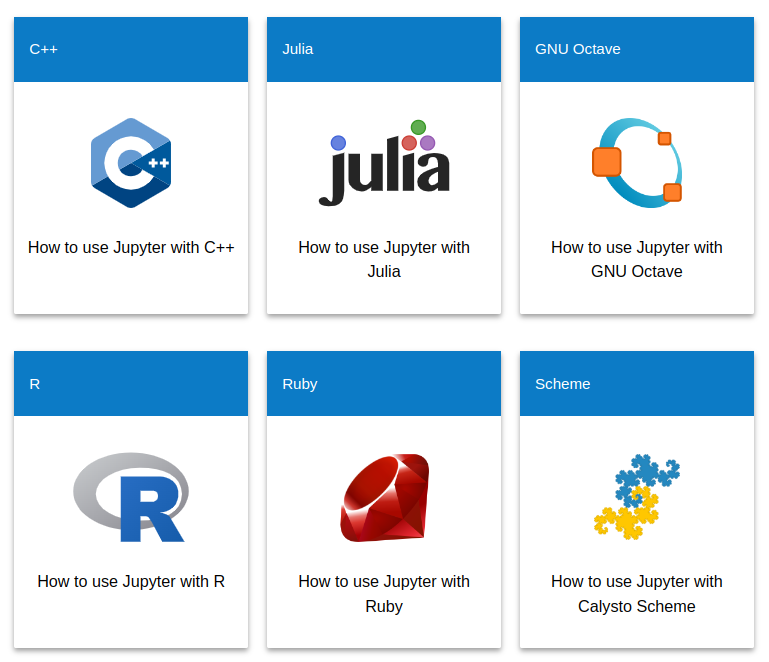
\includegraphics[width=0.5\textwidth]{try-jupyter.png}
  \caption{Calysto Scheme is available online via the Jupyter Project's ``Try Jupyter'' page.}
  \label{fig:try-jupyter}
  \Description{Calysto Scheme, online.}
\end{figure}


%%\begin{figure}
%%  \centering
%%  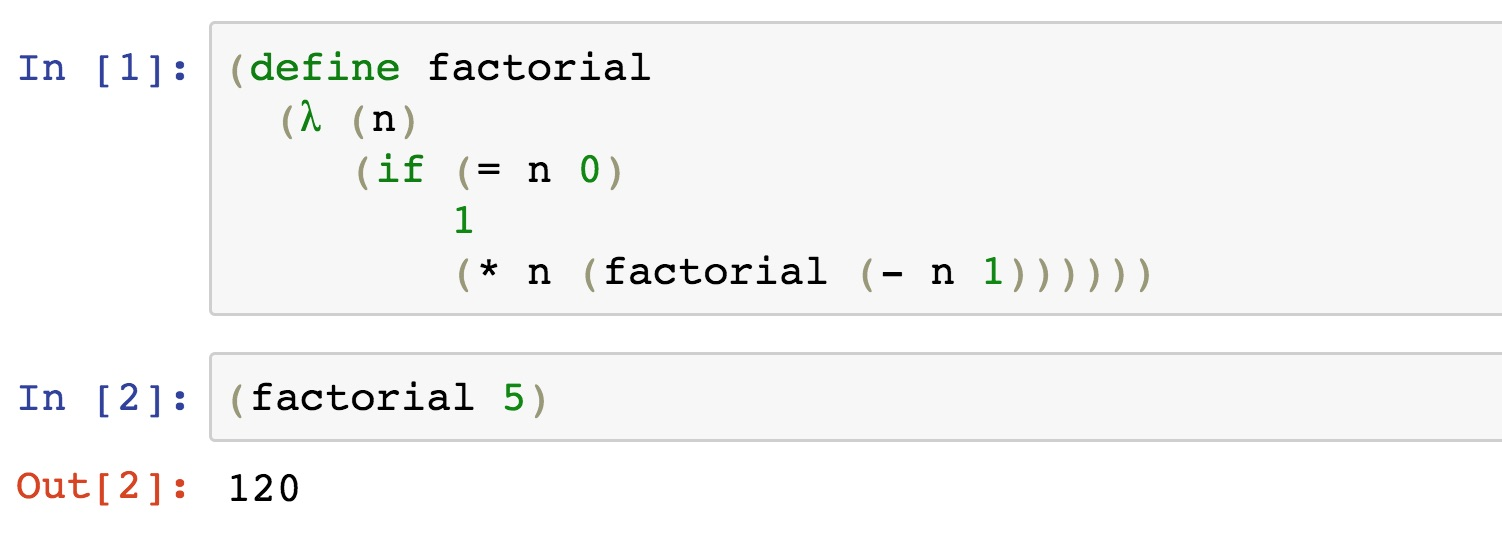
\includegraphics[width=0.6\textwidth]{factorial1.jpg}
%%  \caption{Calysto Scheme running in a Jupyter notebook.}
%%  \label{fig:fact1}
%%  \Description{Calysto Scheme code for the factorial function.}
%%\end{figure}

%%\begin{figure}
%%  \centering
%%  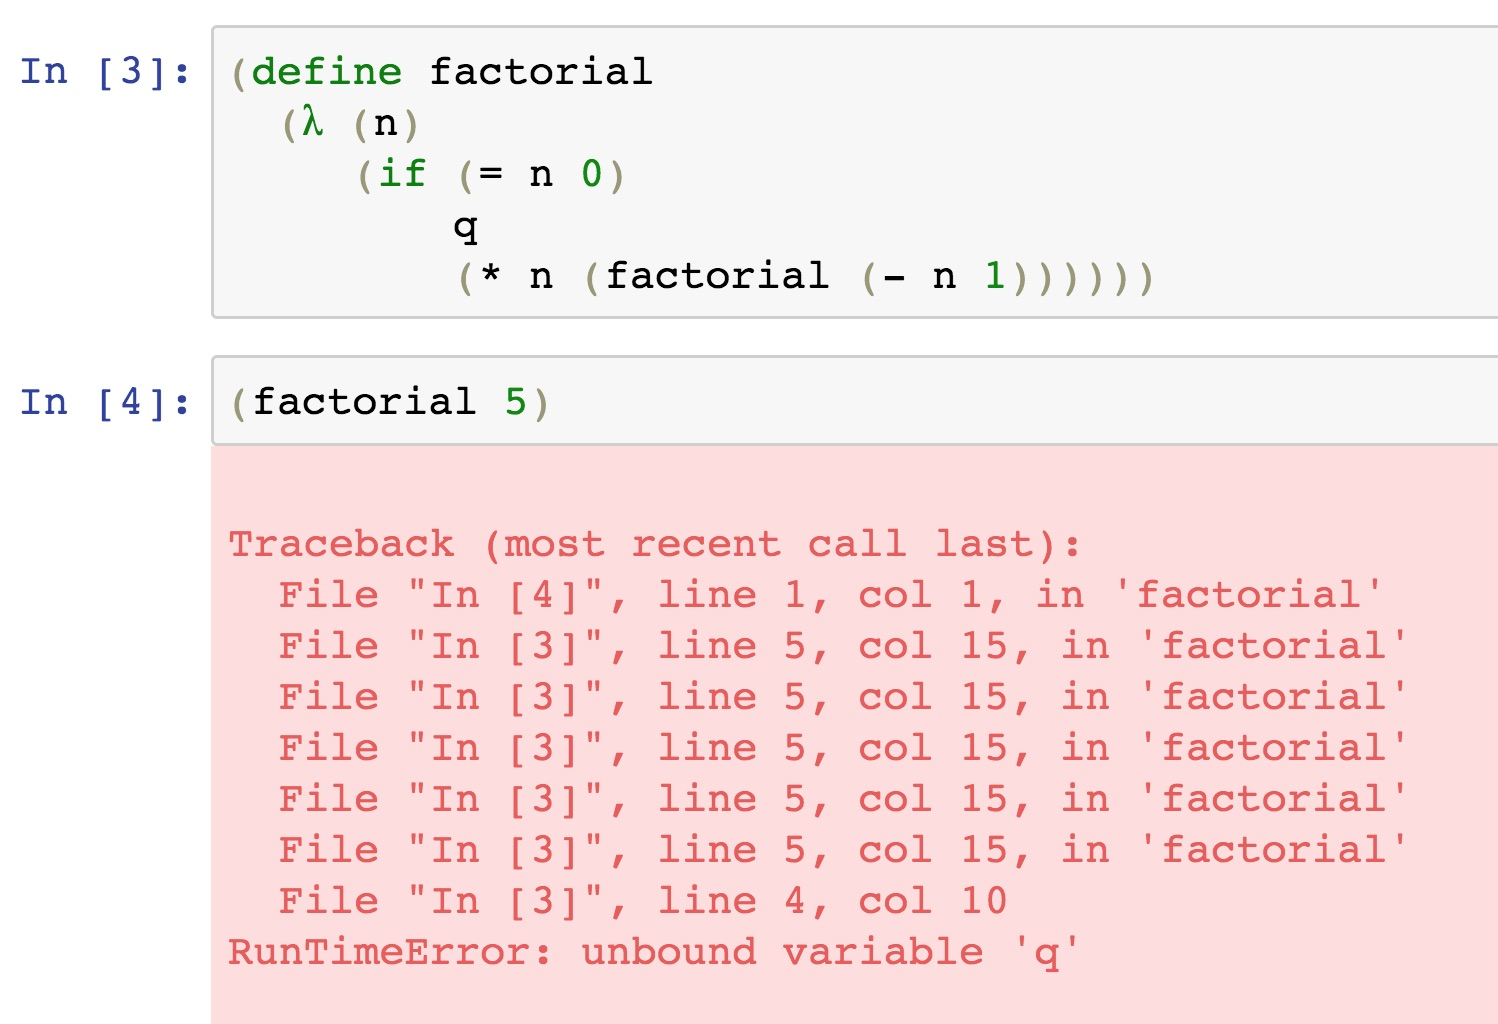
\includegraphics[width=0.6\textwidth]{factorial2.jpg}
%%  \caption{Example of a traceback in Calysto Scheme.}
%%  \label{fig:fact2}
%%  \Description{An error message in the Calysto Scheme programming language.}
%%\end{figure}

\begin{figure}
\begin{minipage}{0.47\textwidth}
  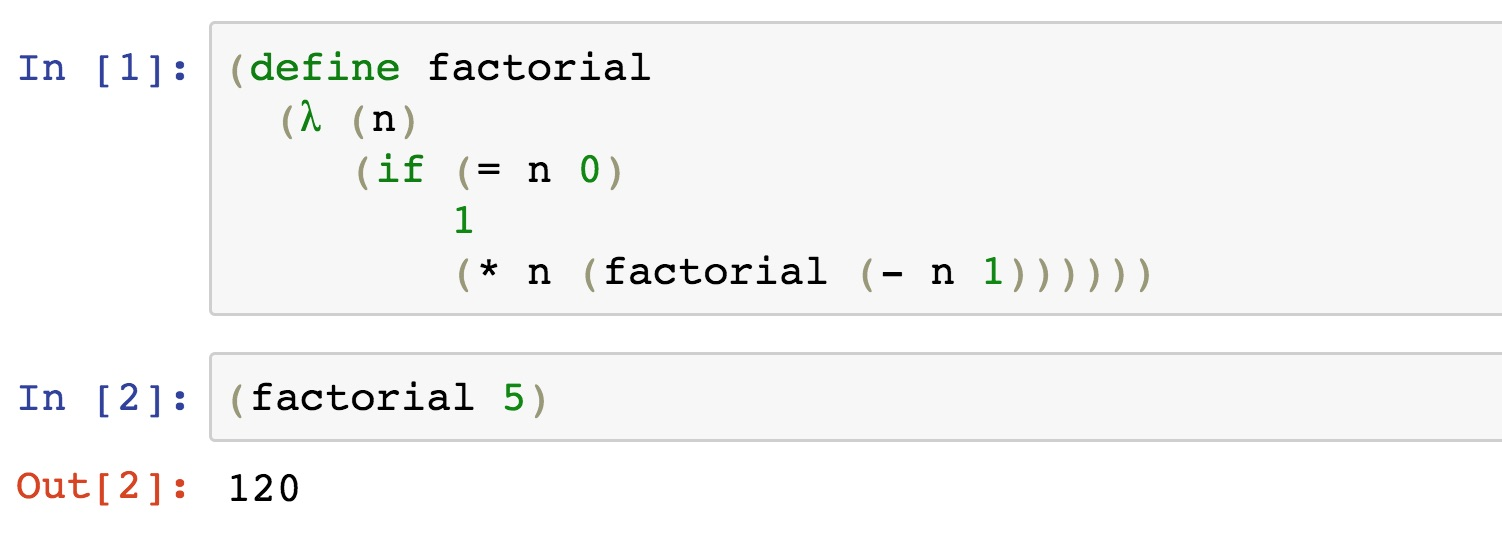
\includegraphics[width=\textwidth]{factorial1.jpg}
  \caption{Calysto Scheme running in a Jupyter notebook.}
  \label{fig:fact1}
  \Description{Calysto Scheme code for the factorial function.}
\end{minipage}
\hspace{0.2in}
\begin{minipage}{0.47\textwidth}
  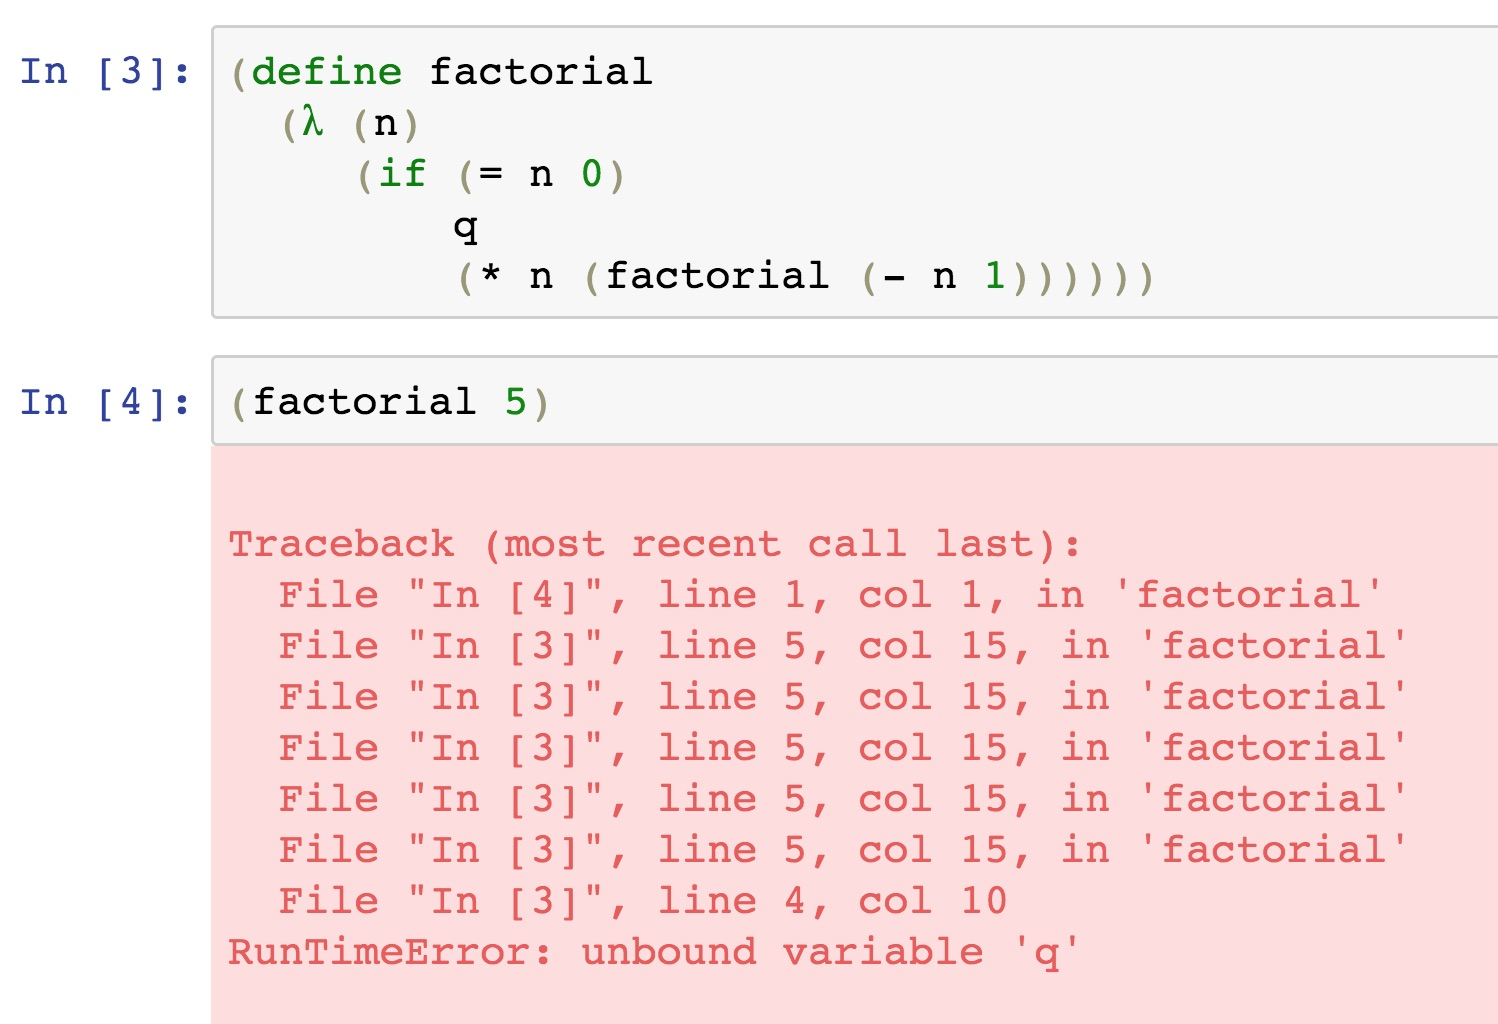
\includegraphics[width=\textwidth]{factorial2.jpg}
  \caption{Example of a traceback in Calysto Scheme.}
  \label{fig:fact2}
  \Description{An error message in the Calysto Scheme programming language.}
\end{minipage}
\end{figure}

\section{Stack-like Tracebacks for Debugging}

In Calysto Scheme, tracebacks are available to help with debugging. For
example, in Figure~\ref{fig:fact2} the definition of the factorial function
contains a typo, with \texttt{q} instead of 1 for the base case, which
generates an unbound variable error. The traceback shows the sequence of
recursive calls that were made before the error occurred. In many Scheme
implementations, since control is not managed with a stack, it is not possible
to generate such a stack trace. However, in Calysto Scheme stack tracing can be
enabled or disabled via the parameter \texttt{use-stack-trace}. For example,
calling \texttt{(use-stack-trace~\#f)} turns off stack tracing.

\section{Scheme in Python, Python in Scheme}

An approach commonly taken in teaching a course in Programming Languages (PL)
is to implement an interpreter for a subset of Scheme in another language, such
as Python. This is a relatively straightforward process, which is considerably
simplified by Scheme's easy-to-parse syntax.  For example, the following code
shows part of an interpreter written in Python with the functions
\texttt{evaluator} and \texttt{apply\_operator} for evaluating Scheme
expressions and applying Scheme functions, respectively:\\

\begin{minipage}{\textwidth}
{\small
\begin{verbatim}
# Scheme-in-Python interpreter

# define parser, reader, tokenizer, and utilities (Map, car, cdr, etc.)

def evaluator(expr):
    if car(expr) == "literal":
        return cadr(expr)
    elif car(expr) == "application":
        return apply_operator(evaluator(cadr(expr)),
                              Map(evaluator, caddr(expr)))
    else:
        raise Exception("Invalid AST: %s" % expr)

def apply_operator(op, operands):
    if op == "+":
        return sum(operands)
    else:
        raise Exception("Unknown operator: %s" % op)

\end{verbatim}
\texttt{evaluator(parser(reader(tokenizer("(+ 1 2)"))))}\\
$\rightarrow$ 3\\
}
\end{minipage}

\noindent
Conversely, one could also teach PL principles by implementing Python in
Scheme. However, this would be much more difficult to attempt in a single
semester course, due to the complexity of Python's syntax. However, if it were
possible to outsource the parsing of Python syntax into Abstract Syntax Tree
(AST) structures, then one could commence with building a Python interpreter
written in Scheme that operates directly on Python ASTs. Because Calysto Scheme
can call Python libraries, this becomes a simple task, as the \texttt{ast}
Python library has the ability to take strings of Python code and turn them
into ASTs \cite{PythonInScheme}.

Mirroring the above Python functions for interpreting Scheme code, one can
easily construct similar functions written in Scheme for interpreting Python
ASTs:\\

\begin{minipage}{\textwidth}
{\small
\begin{verbatim}
;; Python-in-Scheme interpreter

(import "ast")

(define evaluator
  (lambda (ast_expr)
   (cond
     [(isinstance ast_expr ast.Module)
      (evaluator (get-item ast_expr.body 0))]
     [(isinstance ast_expr ast.Num)
      ast_expr.n]
     [(isinstance ast_expr ast.Expr)
      (evaluator ast_expr.value)]
     [(isinstance ast_expr ast.BinOp)
      (apply-operator ast_expr.op
         (evaluator ast_expr.left)
         (evaluator ast_expr.right))]
     [else (error 'evaluator (format "Unknown ast: ~s" ast_expr))])))

(define apply-operator
  (lambda (op v1 v2)
    (cond
      [(isinstance op ast.Add) (+ v1 v2)]
      [else (error 'apply-operator (format "Invalid operator: ~s" op))])))

\end{verbatim}
\texttt{(evaluator (ast.parse "1 + 2"))}\\
$\rightarrow$ 3\\
}
\end{minipage}

\noindent
The main differences between the Scheme interpreter in Python, and the Python
interpreter in Scheme arise from the different ways in which they represent
abstract syntax.  For example, the Scheme expression \texttt{(+~1~2)} is
treated as a function application AST by the Scheme-in-Python interpreter,
whereas the Python expression \texttt{"1~+~2"} is treated as a binary operator
AST by the Python-in-Scheme interpreter.  One could easily change the Scheme
abstract syntax structures to more closely mimic the Python AST structures if
desired, in order to make the two interpreters more parallel.

\section{Summary}

Nothing to see here. Move along.

\begin{acks}
We did it all ourselves.
\end{acks}

\bibliographystyle{ACM-Reference-Format}
\bibliography{scheme2023}

\end{document}
\endinput
